\documentclass[11pt,a4paper,openany]{book}

\PassOptionsToPackage{dvipsnames}{xcolor}
\makeatletter\def\input@path{{../_shared/}}\makeatother
\usepackage{course}

\begin{document}
\raggedbottom

\coursetitle{Intro to Machine Learning}{BA4}{2025--2026}

\tableofcontents
\clearpage

% ============================================================
\chapter{Introduction}
% ============================================================

\section{ML Basics}

\begin{defnbox}[title=Definitions]
\begin{itemize}
    \item \textbf{Data sample}: an individual observation.

    \item \textbf{Data set}: a collection of multiple data samples.

    \item \textbf{Regression}: task on continuous values.

    \item \textbf{Classification}: task on discrete labels.
\end{itemize}
\end{defnbox}

\begin{defnbox}[title=Notations]
\[
x_i \in \mathbb{R}^{D}
\]

It is a column vector of dimension $D$ (the number of features).

\vspace{0.4cm}

\[
y_i \in \mathbb{R}^{C}
\]

It is the target output. For regression, $C = 1$ (a single real value). For multi-class classification with $C$ classes, $y_i$ is a one-hot vector of dimension $C$.

\vspace{0.4cm}

In matrix form, the dataset of $N$ samples is written:
\[
X \in \mathbb{R}^{N \times D}, \qquad y \in \mathbb{R}^{N}
\]
where row $i$ of $X$ is $x_i^T$.
\end{defnbox}

\subsection{Rappels mathématiques}

\begin{rembox}[title=Rappels -- Dérivée et optimalité]
Si on a $R(w)$ une fonction.

\vspace{0.3cm}

\[
R'(\bar{w})
=
\frac{dR}{dw}(\bar{w})
=
\lim_{w \to 0}
\frac{R(\bar{w} + w) - R(\bar{w})}{w}
\]

\vspace{0.3cm}

Si

\[
R'(\bar{w}) = 0
\]

alors cela peut être :
\begin{itemize}
    \item un minimum,
    \item un maximum,
    \item ou un point de selle.
\end{itemize}

On assumera dans la majorité des cas que la solution trouvée sera un minimum.

\vspace{0.3cm}

La solution à partir d'une telle équation, donc le $w$ optimisé, sera dénoté

\[
w^\star
\]
\end{rembox}

\begin{defnbox}[title=Gradient]
Le gradient est la généralisation de la dérivée pour les fonctions multi-variables. Il pointe dans la direction de plus forte augmentation de $R$.

\[
\nabla_{w} R(w)
=
\begin{pmatrix}
\frac{\partial R}{\partial w_1} \\
\frac{\partial R}{\partial w_2} \\
\vdots \\
\frac{\partial R}{\partial w_n}
\end{pmatrix}
\]

\vspace{0.3cm}

Si le gradient est égal au vecteur nul :

\[
\nabla_w R(w) = 0
\]

alors on obtient un \textit{stationary point} lorsque l'on recherche $w^\star$.
\end{defnbox}

\begin{propbox}[title=Useful Identities]
\[
\nabla_b (a^T b) = a
\]

\[
\|a\|^2 = a^T a
\]

\[
\nabla_a \|a\|^2 = 2a
\]

\[
\nabla_B (a^T B) = a
\]
\end{propbox}

% ============================================================
\chapter{Linear Supervised ML}
% ============================================================

\section{Linear regression}

\begin{rembox}[title=Pourquoi et quand utiliser la régression linéaire ?]
\textbf{Pourquoi :} La régression linéaire est le modèle le plus simple pour prédire une valeur continue. Elle a une solution analytique exacte (pas besoin d'itérations), est rapide à entraîner, et ses paramètres sont facilement interprétables.

\vspace{0.3cm}

\textbf{Quand :} On l'utilise lorsque la relation entre les features $x_i$ et la cible $y_i$ est approximativement linéaire, et que la sortie est une valeur continue (ex : prédire un prix, une température).

\vspace{0.3cm}

\textbf{Output :} Un scalaire $\hat{y}_i \in \mathbb{R}$ (ou un vecteur pour le multi-output).
\end{rembox}

Le principe de la régression linéaire est d'essayer de fitter une droite, un plan, ou un hyperplan sur les données que nous avons afin de pouvoir en faire des approximations.

\vspace{0.4cm}

\subsection{Train}

On cherche à trouver le vecteur $w$ optimal tel que :

\[
\hat{y}_i = w^T x_i
\]

Pour trouver ce $w$, on cherche le $w$ optimal noté $w^\star$, tel que les prédictions soient les plus proches des vraies valeurs.

\vspace{0.6cm}

\begin{defnbox}[title=Measure of closeness]
Pour mesurer la distance entre la prédiction et la réalité, on utilise la distance euclidienne :

\[
d(\hat{y}_i, y_i) = \sqrt{(\hat{y}_i - y_i)^2}
\]

En pratique, on utilise la squared Euclidean distance :

\[
d^2(\hat{y}_i, y_i) = (\hat{y}_i - y_i)^2
\]

Comme la racine carrée est monotone croissante sur les réels positifs, minimiser la distance ou son carré revient au même. Utiliser le carré a aussi l'avantage de rendre la fonction différentiable et de pénaliser plus fortement les grandes erreurs.

\vspace{0.4cm}
\end{defnbox}

\vspace{0.4cm}

On va alors chercher à minimiser cette distance, pour être le plus proche possible des vrais résultats.
Le training devient donc un minimization problem où on va tenter de minimiser ce que l'on définit comme la fonction de coût (empirical risk) :

\[
R(w) = \frac{1}{N} \sum_{i=1}^{N} (w^T x_i - y_i)^2
\]

Le problème de training devient donc :

\[
\min_w R(w)
\]

\vspace{0.6cm}

\begin{defnbox}[title=Empirical Risk]
La \textbf{empirical risk} $R(w)$ mesure l'erreur moyenne du modèle sur les données d'entraînement. Sa forme générale est :

\[
R(\{x_i\}, \{y_i\}, w)
=
\frac{1}{N} \sum_{i=1}^{N} \ell(\hat{y}_i, y_i)
\]

où $\ell$ est la \textit{loss function} (fonction de perte). En régression linéaire, on utilise $\ell(\hat{y}, y) = (\hat{y} - y)^2$.
\end{defnbox}

\vspace{1.0cm}

Pour minimiser $R(w)$, on calcule le gradient et on impose qu'il soit nul.
On applique la dérivation terme à terme :

\[
\nabla_w R(w)
=
\frac{1}{N} \sum_{i=1}^{N} \nabla_w \big( (w^T x_i - y_i)^2 \big)
\]

\vspace{0.4cm}

En utilisant la règle de la chaîne :

\[
\nabla_w (u^2) = 2u \, \nabla_w u
\]

avec \( u = w^T x_i - y_i \), et en notant que \( \nabla_w (w^T x_i) = x_i \), on obtient :

\[
\nabla_w R(w)
=
\frac{2}{N} \sum_{i=1}^{N} (w^T x_i - y_i)x_i
\]

On impose la condition d'optimalité :

\[
\nabla_w R(w) = 0
\]

Ce qui donne :

\[
\sum_{i=1}^{N} x_i x_i^T w^\star = \sum_{i=1}^{N} x_i y_i
\]

\vspace{0.4cm}

\textbf{Forme matricielle :}

\[
X^T X w^\star = X^T y
\]

\vspace{0.4cm}

Si $X^T X$ est inversible :

\[
w^\star = (X^T X)^{-1} X^T y
\]

Sinon (cas sous-déterminé ou sur-déterminé), on utilise la pseudo-inverse :

\[
w^\star = X^\dagger y
\]

\vspace{0.8cm}

\subsection{Test}

Une fois le modèle entraîné, on prédit sur un nouveau point $x$ :

\[
\hat{y} = w^{\star T} x
\]

\textbf{Output :} un scalaire $\hat{y} \in \mathbb{R}$.

\vspace{0.8cm}

\subsection{Complement: multiple outputs}

On généralise à plusieurs sorties ($C > 1$) :

\[
\min_W \sum_{i=1}^{N} \|W^T x_i - y_i\|^2
\]

avec :

\[
W = [w_1 \; w_2 \; \dots \; w_C] \in \mathbb{R}^{D \times C}
\]

Chaque colonne $w_k$ prédit la $k$-ème sortie indépendamment. La solution devient :

\[
W^\star = X^\dagger Y
\]

\vspace{0.8cm}

\textbf{Conclusion :}

La régression linéaire permet d'obtenir une solution fermée exacte grâce à l'optimisation d'une fonction de coût quadratique convexe. Cela garantit que le minimum trouvé correspond à l'optimum global.

Ainsi, une fois $W^\star$ calculé, la phase de test consiste simplement à appliquer :

\[
\hat{y} = W^{\star T} x
\]

\vspace{0.4cm}

Le modèle est donc entièrement déterminé par la solution analytique du problème d'optimisation.

\vspace{8cm}

\subsection{Model evaluation on test sample}

Après training, il faut mesurer si le modèle est bon sur des données qu'il n'a pas vues.
On utilise pour cela des métriques calculées sur le jeu de test.

\vspace{0.6cm}

\begin{defnbox}[title=Mean Squared Error (MSE)]
Moyenne des erreurs au carré. Pénalise fortement les grandes erreurs.

\[
\mathrm{MSE} = \frac{1}{N} \sum_{i=1}^{N} (y_i - \hat{y}_i)^2
\]
\end{defnbox}

\vspace{0.4cm}

\begin{defnbox}[title=Root Mean Squared Error (RMSE)]
Racine carrée du MSE. Exprimée dans la même unité que $y_i$, donc plus interprétable.

\[
\mathrm{RMSE} = \sqrt{\frac{1}{N} \sum_{i=1}^{N} (y_i - \hat{y}_i)^2}
\]
\end{defnbox}

\vspace{0.4cm}

\begin{defnbox}[title=Mean Absolute Error (MAE)]
Moyenne des erreurs absolues. Moins sensible aux outliers que le MSE.

\[
\mathrm{MAE} = \frac{1}{N} \sum_{i=1}^{N} |\hat{y}_i - y_i|
\]
\end{defnbox}

\vspace{0.4cm}

\begin{defnbox}[title=Mean Absolute Percentage Error (MAPE)]
Erreur relative en pourcentage. Utile pour comparer des modèles sur des cibles d'échelles différentes. Attention : ne fonctionne pas si $y_i = 0$.

\[
\mathrm{MAPE} = \frac{1}{N} \sum_{i=1}^{N} \left| \frac{\hat{y}_i - y_i}{y_i} \right|
\]
\end{defnbox}

% ------------------------------------------------------------
\newpage \section{Linear models for classification}
% ------------------------------------------------------------

\vspace{8cm}


\subsection{Logistic Regression}

\begin{rembox}[title=Pourquoi et quand utiliser la logistic regression ?]
\textbf{Pourquoi :} On ne peut pas utiliser directement la régression linéaire pour la classification car ses prédictions $w^T x_i$ peuvent prendre n'importe quelle valeur dans $\mathbb{R}$, alors qu'on cherche une probabilité dans $[0, 1]$. La logistic regression résout ce problème en passant la prédiction linéaire à travers une fonction sigmoid.

\vspace{0.3cm}

\textbf{Quand :} Problème de classification binaire (2 classes) avec des données approximativement linéairement séparables dans l'espace des features.

\vspace{0.3cm}

\textbf{Output :} Une probabilité $\hat{y}_i \in (0, 1)$ interprétée comme $p(\text{class} = 1 \mid x_i)$, puis un label $\{0, 1\}$ par seuillage.
\end{rembox}

\vspace{0.6cm}

\subsubsection{Pourquoi pas la linear regression pour classifier ?}

On pourrait utiliser la régression linéaire pour un problème de classification en seuillant le résultat :

\[
\hat{y} =
\begin{cases}
1 & \text{if } w^T x \geq 0.5 \\
0 & \text{otherwise}
\end{cases}
\]

Mais cette méthode n'est pas fiable : les prédictions ne sont pas des probabilités, et la fonction de perte quadratique pénalise les points bien classifiés mais éloignés de la frontière.

\vspace{0.8cm}

\subsubsection{Logistic Sigmoid Function}

Pour obtenir une probabilité, on applique la \textbf{sigmoid function} à la combinaison linéaire $w^T x_i$ :

\vspace{0.4cm}

\begin{defnbox}[title=Sigmoid function]
\[
\sigma(z) = \frac{1}{1 + e^{-z}} \in (0, 1)
\]

Elle mappe $\mathbb{R} \to (0,1)$, ce qui permet d'interpréter la sortie comme une probabilité.
\end{defnbox}

\vspace{0.4cm}

Dans notre cas, la prédiction devient :

\[
\hat{y}_i = \sigma(w^T x_i) = \frac{1}{1 + \exp(-w^T x_i)}
\]

\vspace{0.8cm}

\subsubsection{Training}

On veut trouver $w^\star$ qui maximise la vraisemblance des observations. Pour un sample $i$ de label $y_i \in \{0,1\}$, la probabilité du label donné $w$ est :

\[
p(y_i | x_i, w) = \hat{y}_i^{y_i} (1 - \hat{y}_i)^{1 - y_i}
\]

Sur tout le dataset (échantillons supposés indépendants) :

\[
p(y|w) = \prod_{i=1}^{N} \hat{y}_i^{y_i} (1 - \hat{y}_i)^{1 - y_i}
\]

\vspace{0.4cm}

En prenant le log (pour transformer le produit en somme) et en passant à la minimisation (on minimise le négatif), on obtient la \textbf{binary cross-entropy loss} :

\[
R(w) =
- \sum_{i=1}^{N} \Big( y_i \ln(\hat{y}_i) + (1 - y_i)\ln(1 - \hat{y}_i) \Big)
\]

\vspace{0.4cm}

Interprétation :
\begin{itemize}
    \item Pour les samples positifs ($y_i = 1$) : on veut maximiser $\ln(\hat{y}_i)$, donc on pénalise si $\hat{y}_i$ est faible.
    \item Pour les samples négatifs ($y_i = 0$) : on veut maximiser $\ln(1 - \hat{y}_i)$, donc on pénalise si $\hat{y}_i$ est élevé.
\end{itemize}

\vspace{0.4cm}

Contrairement à la régression linéaire, il n'existe pas de solution fermée. On utilise donc le \textbf{gradient descent}.

\vspace{0.6cm}

Le gradient se calcule en séparant positifs et négatifs puis en les réunissant :

\[
\nabla_w R(w)
=
\sum_{i=1}^{N} (\hat{y}_i - y_i)x_i
\]

\vspace{0.8cm}

\begin{algbox}[title=Gradient Descent Algorithm]
\textbf{But :} minimiser $R(w)$ de façon itérative en descendant dans la direction opposée au gradient.

\vspace{0.3cm}

1. Initialize $w_0$ randomly

2. While not converged:

\[
w_k \leftarrow w_{k-1} - \eta \, \nabla_w R(w_{k-1})
\]

\vspace{0.4cm}

\begin{itemize}
    \item $\eta > 0$ est le \textbf{learning rate} : trop grand $\Rightarrow$ divergence ; trop petit $\Rightarrow$ convergence lente.
    \item À chaque itération, on se rapproche du minimum de $R$.
\end{itemize}
\end{algbox}

\begin{rembox}[title=Convergence criteria]
On arrête lorsqu'une des conditions suivantes est satisfaite :
\begin{itemize}
    \item $|R(w_k) - R(w_{k-1})| < \delta_R$ \quad (la loss ne bouge plus)
    \item $\|w_k - w_{k-1}\| < \delta_w$ \quad (les paramètres ne bougent plus)
    \item Nombre fixe d'itérations atteint (budget computationnel)
\end{itemize}
\end{rembox}

\vspace{0.8cm}

\subsubsection{Test}

Une fois $w^\star$ trouvé :

\[
\hat{y}_i = \sigma(w^{\star T} x_i)
\]

Puis classification par seuillage :

\[
\text{label} =
\begin{cases}
1 & \text{if } \hat{y}_i \geq 0.5 \\
0 & \text{otherwise}
\end{cases}
\]

Le seuil $0.5$ peut être ajusté selon le contexte (ex : priorité à la précision ou au recall).
\vspace{8cm}

\subsection{Classification evaluation}

Après entraînement, comment savoir si le modèle classifie correctement ?
On compare les labels prédits aux labels réels via une \textbf{confusion matrix} (pour 2 classes, c'est un tableau $2\times 2$) :

\vspace{0.4cm}

\begin{center}
\renewcommand{\arraystretch}{1.6}
\setlength{\tabcolsep}{12pt}

\begin{tabular}{c|c|c}
\multicolumn{1}{c}{} & \multicolumn{2}{c}{\textbf{True class}} \\
\cline{2-3}
\textbf{Predicted class} & Pos & Neg \\
\hline
Pos & TP & FP \\
Neg & FN & TN \\
\end{tabular}
\end{center}

\vspace{0.4cm}

\begin{itemize}
    \item \textbf{TP} (True Positive) : prédit positif, vrai label positif.
    \item \textbf{TN} (True Negative) : prédit négatif, vrai label négatif.
    \item \textbf{FP} (False Positive, type I error) : prédit positif, vrai label négatif.
    \item \textbf{FN} (False Negative, type II error) : prédit négatif, vrai label positif.
\end{itemize}

\vspace{0.4cm}

\[
P = TP + FN \quad \text{(total real positives)}
\qquad
N = FP + TN \quad \text{(total real negatives)}
\]

\vspace{0.8cm}

\begin{defnbox}[title=Accuracy]
\textbf{Definition:} proportion of correctly classified samples (all classes combined).

\[
\mathrm{Accuracy} = \frac{TP + TN}{TP + TN + FP + FN}
\]

\textbf{Limitation :} trompeuse sur des données déséquilibrées (ex : 99\% de négatifs $\Rightarrow$ prédire toujours négatif donne 99\% d'accuracy).
\end{defnbox}

\vspace{0.4cm}

\begin{defnbox}[title=Precision]
\textbf{Definition:} parmi tout ce qui a été prédit positif, quelle fraction l'est vraiment ?

\[
\mathrm{Precision} = \frac{TP}{TP + FP}
\]

\textbf{Quand la prioriser :} quand les fausses alarmes sont coûteuses (ex : spam filter).
\end{defnbox}

\vspace{0.4cm}

\begin{defnbox}[title=Recall (Sensitivity)]
\textbf{Definition:} parmi tous les vrais positifs, quelle fraction a été détectée ?

\[
\mathrm{Recall} = \frac{TP}{TP + FN}
\]

\textbf{Quand le prioriser :} quand manquer un positif est coûteux (ex : détection de cancer).
\end{defnbox}

\vspace{0.4cm}

\begin{defnbox}[title=False Positive Rate (FPR)]
\textbf{Definition:} proportion de négatifs incorrectement classifiés comme positifs.

\[
\mathrm{FPR} = \frac{FP}{FP + TN}
\]
\end{defnbox}

\vspace{0.4cm}

\begin{defnbox}[title=F1 Score]
La précision et le recall sont souvent en tension (améliorer l'un dégrade l'autre). Le F1-score est leur moyenne harmonique :

\[
\mathrm{F1} = 2 \cdot \frac{\mathrm{Precision} \cdot \mathrm{Recall}}{\mathrm{Precision} + \mathrm{Recall}}
\]

\vspace{0.3cm}

\textbf{Interpretation:} The F1-score ranges between $0$ and $1$.

\begin{itemize}
    \item $F1 \approx 1$ : excellent balance between precision and recall
    \item $F1 \approx 0.5$ : imbalance between precision and recall
    \item $F1 \approx 0$ : very poor model
\end{itemize}

\textbf{Quand l'utiliser :} données déséquilibrées où l'accuracy est trompeuse.
\end{defnbox}
\vspace{8cm}

\subsection{Dealing with multi class}

Maintenant, ce qu'on a fait pour la classification marchait seulement si on devait choisir entre 2 classes.
Mais comment fait-on lorsque l'on a $C > 2$ classes ?

\vspace{0.5cm}

On représente alors les labels différemment avec le \textbf{one-hot encoding} :
$y_i$ devient un vecteur de dimension $C$ contenant des $0$ et un unique $1$ à la position correspondant au label.

\vspace{0.5cm}

Exemple pour $C = 7$ classes, label = classe 3 :

\[
y_i =
\begin{pmatrix}
0 \\ 0 \\ 0 \\ 1 \\ 0 \\ 0 \\ 0
\end{pmatrix}
\]

\vspace{0.8cm}

\subsubsection{Linear classification (multi-class)}

La méthode de train devient un problème de régression multi-output :

\[
\min_W \sum_{i=1}^{N} \|W^T x_i - y_i\|^2
\]

\vspace{0.4cm}

dont la solution est :

\[
W^\star = X^\dagger Y
\]

\vspace{0.4cm}

Pour prédire, on calcule un score pour chaque classe :

\[
\hat{y}_i = W^{\star T} x_i \in \mathbb{R}^C
\]

\vspace{0.5cm}

On choisit la classe ayant le score le plus élevé :

\[
k =
\underset{j}{\arg\max}
\;
\hat{y}_i^{(j)}
\]

\vspace{0.8cm}

\subsubsection{Logistic regression (multi-class -- Softmax)}

On remplace la fonction sigmoid par la \textbf{Softmax} qui généralise sigmoid à $C$ classes.
La Softmax produit une distribution de probabilité sur toutes les classes (les valeurs sont dans $(0,1)$ et leur somme est $1$) :

\[
\hat{y}^{(k)}(x)
=
\frac{
\exp\left(w^{(k)T}x\right)
}{
\sum_{j=1}^{C}
\exp\left(w^{(j)T}x\right)
}
\]

\vspace{0.5cm}

Avec :

\begin{itemize}
    \item $w^{(k)}$ : la $k$-ème colonne de $W$ (poids pour la classe $k$)
    \item $C$ : le nombre de classes
    \item $\hat{y}^{(k)}(x) \approx p(\text{class} = k \mid x)$
\end{itemize}

\vspace{0.6cm}

L'empirical risk devient la \textbf{cross-entropy loss} multi-classe :

\[
R(W)
=
-
\sum_{i=1}^{N}
\sum_{k=1}^{C}
y_i^{(k)}
\ln\left(\hat{y}_i^{(k)}\right)
\]

\vspace{0.6cm}

Et on applique le gradient descent avec :

\[
\nabla_W R(W)
=
\sum_{i=1}^{N}
x_i
(\hat{y}_i - y_i)^T
\]

\vspace{0.8cm}

Le résultat final est obtenu par :

\[
k =
\underset{j}{\arg\max}
\;
\hat{y}^{(j)}(x)
\]

\vspace{8cm}

\subsection{Evaluation metrics on multi-class classification}

Avec plusieurs classes, on généralise la confusion matrix en un tableau $C \times C$.

\vspace{0.6cm}

\begin{exbox}[title=Confusion matrix -- 3 classes]
\[
\begin{array}{c|c|c|c}
& \text{True A} & \text{True B} & \text{True C} \\
\hline
\text{Predicted A} & \cdots & \cdots & \cdots \\
\hline
\text{Predicted B} & \cdots & \cdots & \cdots \\
\hline
\text{Predicted C} & \cdots & \cdots & \cdots \\
\end{array}
\]

\vspace{0.4cm}

La diagonale contient les bons classements. Les éléments hors-diagonale sont des erreurs.
\end{exbox}

\vspace{0.8cm}

L'Accuracy se généralise directement :

\[
\mathrm{Accuracy}
=
\frac{
\sum_{k=1}^{C} \text{true positives for class } k
}{
\text{total samples}
}
\]

\vspace{0.8cm}

Pour Precision, Recall, FPR et F1-score, on calcule la métrique pour chaque classe (one-vs-all) puis on en fait la moyenne.

\vspace{0.4cm}

\begin{rembox}[title=Macro vs Weighted Average]
\begin{itemize}
    \item \textbf{Macro average} : moyenne simple sur toutes les classes. Chaque classe contribue également, quelle que soit sa taille.

    \item \textbf{Weighted average} : moyenne pondérée par le nombre de samples par classe. Prend en compte le déséquilibre des classes (\textit{class imbalance}).
\end{itemize}

En pratique, si les classes sont déséquilibrées, préférer le \textbf{weighted average} ou l'analyse par classe séparément.
\end{rembox}

\vspace{8cm}

\subsection{SVM -- Support Vector Machines}

\begin{rembox}[title=Pourquoi et quand utiliser les SVM ?]
\textbf{Pourquoi :} La logistic regression trouve \textit{une} frontière qui sépare les classes, mais pas nécessairement la \textit{meilleure}. Les SVM cherchent la frontière qui maximise la marge (distance aux points les plus proches), ce qui améliore la généralisation.

\vspace{0.3cm}

\textbf{Quand :} Classification binaire, surtout quand les données sont linéairement séparables ou presque. Très efficace en haute dimension. S'étend aux problèmes non-linéaires via les kernels.

\vspace{0.3cm}

\textbf{Output :} Un label binaire $\hat{y} \in \{-1, +1\}$.
\end{rembox}

\vspace{0.5cm}

\subsubsection{Intuition}

On cherche un hyperplan $w^T x + b = 0$ qui sépare les deux classes ($y_i \in \{-1, +1\}$).
Parmi tous les hyperplans qui séparent correctement les données, on choisit celui qui maximise la marge.

\vspace{0.5cm}

\begin{defnbox}[title=Margin]
La marge est la distance minimale entre l'hyperplan et les points les plus proches de chaque classe.

\[
\text{margin} = \frac{2}{\|w\|}
\]

Les points qui définissent la marge (les plus proches de l'hyperplan) sont appelés les \textbf{support vectors}.
\end{defnbox}

\vspace{0.6cm}

\subsubsection{Hard-margin SVM (données linéairement séparables)}

On maximise la marge sous contrainte que tous les points soient correctement classifiés :

\[
\min_{w, b} \frac{1}{2} \|w\|^2
\quad \text{s.t.} \quad
y_i (w^T x_i + b) \geq 1 \quad \forall i
\]

La contrainte $y_i (w^T x_i + b) \geq 1$ force chaque point à être du bon côté de la marge.

\vspace{0.6cm}

\subsubsection{Soft-margin SVM (données non parfaitement séparables)}

En pratique, les données ne sont pas toujours linéairement séparables.
On introduit des \textbf{slack variables} $\xi_i \geq 0$ qui permettent à certains points de violer la marge :

\[
\min_{w, b, \xi} \frac{1}{2} \|w\|^2 + C \sum_{i=1}^{N} \xi_i
\quad \text{s.t.} \quad
y_i (w^T x_i + b) \geq 1 - \xi_i, \quad \xi_i \geq 0 \quad \forall i
\]

Avec :
\begin{itemize}
    \item $C > 0$ : hyperparamètre contrôlant le compromis entre marge large et erreurs tolérées.
    \item $C$ grand $\Rightarrow$ peu d'erreurs tolérées (risque d'overfitting).
    \item $C$ petit $\Rightarrow$ marge plus large mais plus d'erreurs (risque d'underfitting).
\end{itemize}

\vspace{0.6cm}

\subsubsection{Prédiction}

\[
\hat{y} = \text{sign}(w^T x + b) \in \{-1, +1\}
\]

\vspace{0.6cm}

\subsubsection{Regularization built-in}

Le terme $\frac{1}{2}\|w\|^2$ dans l'objectif joue le rôle d'une régularisation L2, qui pénalise les poids trop grands. C'est pourquoi les SVM n'ont pas besoin d'un terme de régularisation additionnel explicite.

\vspace{0.6cm}

\subsubsection{Kernel SVM}

Pour des données non-linéairement séparables, on peut kerneliser le SVM en remplaçant le produit scalaire $x_i^T x_j$ par un kernel $k(x_i, x_j)$ dans la formulation duale. Cela revient à travailler dans un espace de features de grande dimension sans le calculer explicitement.

% ============================================================
\chapter{Non-linear Supervised ML}
% ============================================================
\vspace{8cm}

\section{k-Nearest Neighbors}

\begin{rembox}[title=Pourquoi et quand utiliser KNN ?]
\textbf{Pourquoi :} KNN est un algorithme non-paramétrique : il ne fait aucune hypothèse sur la forme des données. Il mémorise l'ensemble du training set et prédit en cherchant les points les plus similaires.

\vspace{0.3cm}

\textbf{Quand :} Données avec des frontières de décision complexes et non-linéaires. Fonctionne bien sur de petits datasets. Simple à implémenter et sans phase d'entraînement.

\vspace{0.3cm}

\textbf{Limitations :} Prédiction lente (distance à tous les points de training à chaque fois). Sensible aux features mal scalées et aux outliers. Pas adapté aux grands datasets.

\vspace{0.3cm}

\textbf{Output :} Un label de classe (classification) ou une valeur continue (régression).
\end{rembox}

\vspace{0.8cm}

\subsection{Distances}

Pour déterminer les voisins les plus proches, on choisit une mesure de distance.
Le choix de la distance dépend de la nature des données.

\vspace{0.5cm}

\begin{defnbox}[title=Euclidian distance]
Mesure standard de la distance géométrique entre deux points. Adaptée aux features continues de même échelle.

\[
d(x_i, x_j)
=
\sqrt{
\sum_{k=1}^{D}
(x_i^{(k)} - x_j^{(k)})^2
}
\]
\end{defnbox}

\vspace{0.5cm}

\begin{defnbox}[title=Chi-square distance]
Distance souvent utilisée pour comparer des distributions ou histogrammes (ex : features de fréquence).

\[
d(x_i, x_j)
=
\sqrt{\chi^2(x_i, x_j)}
=
\sqrt{
\sum_{k=1}^{D}
\frac{
\left(x_i^{(k)} - x_j^{(k)}\right)^2
}{
x_i^{(k)} + x_j^{(k)}
}
}
\]
\end{defnbox}

\vspace{0.8cm}

\subsection{Classification}

Pour la classification : on prend le vote majoritaire parmi les $k$ voisins les plus proches.

\vspace{0.5cm}

\begin{algbox}[title=KNN classification algorithm]
\begin{enumerate}
    \item Compute distance between $x$ and all $x_i$ in the training set

    \item Find the $k$ samples with minimum distances

    \item Find the most common label among these $k$ nearest neighbors (majority vote)

    \item Assign that label as $\hat{y}$
\end{enumerate}
\end{algbox}

\begin{rembox}[title=Choix de $k$]
\begin{itemize}
    \item $k = 1$ : modèle très flexible, risque d'overfitting.
    \item $k$ grand : modèle plus lisse, risque d'underfitting.
    \item On choisit $k$ par cross-validation.
    \item En pratique, choisir $k$ impair pour éviter les égalités (pour 2 classes).
\end{itemize}
\end{rembox}

\vspace{0.8cm}

\subsection{Regression}

Pour la régression : on fait la moyenne (éventuellement pondérée) des valeurs des $k$ voisins.

\vspace{0.5cm}

\begin{algbox}[title=KNN regression algorithm]
\begin{enumerate}
    \item Compute distance between $x$ and all $x_i$

    \item Find $k$ samples with minimum distances

    \item Compute the predicted value as a (weighted) average of the neighbors:

    \[
    \hat{y}
    =
    \frac{
    \sum_i w_i y_i
    }{
    \sum_i w_i
    }
    \]

    avec $w_i = 1$ (unweighted) ou $w_i = \frac{1}{d_i}$ (inverse distance weighting : les voisins plus proches ont plus d'influence).

\end{enumerate}
\end{algbox}

% ------------------------------------------------------------
\newpage \section{Feature expansion}
% ------------------------------------------------------------
\vspace{8cm}

\subsection{Polynomial curve fitting}

\begin{rembox}[title=Pourquoi et quand utiliser la feature expansion ?]
\textbf{Pourquoi :} Les modèles linéaires ne peuvent capturer que des relations linéaires entre les features et la cible. Si les données suivent une courbe, un cercle, ou un polynôme complexe, un modèle linéaire sera trop limité. La feature expansion transforme les features pour rendre les relations non-linéaires linéairement représentables.

\vspace{0.3cm}

\textbf{Quand :} Les données ont une structure non-linéaire dans l'espace original, mais on veut garder la simplicité et la tractabilité des modèles linéaires.

\vspace{0.3cm}

\textbf{Output :} Le même type de sortie que le modèle linéaire sous-jacent, mais avec une frontière de décision non-linéaire dans l'espace original.
\end{rembox}

\vspace{0.8cm}

\subsubsection{Principe}

On prend nos données de base $x$ puis on leur applique une transformation $\phi$ qui crée un nouveau vecteur contenant différentes combinaisons (polynomiales) des features initiales.

\vspace{0.5cm}

Par exemple :

\[
x =
\begin{pmatrix}
x_1 \\
x_2
\end{pmatrix}
\]

\vspace{0.4cm}

Après polynomial curve expansion (degré 2) :

\[
\phi(x)
=
\begin{pmatrix}
1 \\
x_1 \\
x_2 \\
x_1^2 \\
x_1 x_2 \\
x_2^2
\end{pmatrix}
\]

\vspace{0.5cm}

On obtient alors un modèle encore linéaire \textit{dans l'espace transformé}, mais non-linéaire dans l'espace original :

\[
\hat{y}_i = w^T \phi(x_i)
\]

\vspace{0.4cm}

Avec :

\begin{itemize}
    \item $\phi(x_i) \in \mathbb{R}^{F}$ (où $F$ est le nombre de features après expansion)
    \item $w \in \mathbb{R}^{F}$
\end{itemize}

\vspace{0.8cm}

\subsubsection{Solution analytique}

On obtient alors le gradient :

\[
\nabla_w R(w)
=
2
\sum_{i=1}^{N}
\phi(x_i)
\left(
\phi(x_i)^T w - y_i
\right)
\]

\vspace{0.6cm}

En imposant $\nabla_w R(w) = 0$, on obtient :

\[
w^\star
=
(\Phi^T \Phi)^{-1}\Phi^T y
\]

où $\Phi \in \mathbb{R}^{N \times F}$ est la matrice dont la ligne $i$ est $\phi(x_i)^T$.

\begin{thmbox}[title=Cover's theorem]
\textit{
A complex pattern classification problem cast in a high-dimensional space non-linearly is more likely to be linearly separable than in a low-dimensional space, provided that the space is not densely populated.
}

\vspace{0.3cm}

En d'autres termes : en augmentant la dimensionnalité via $\phi$, on facilite la séparation linéaire des classes.
\end{thmbox}
\vspace{8cm}

\subsection{Fitting and regularization -- Cross validation}

\begin{defnbox}[title=Definition: Overfitting]
Le modèle mémorise les données d'entraînement mais ne généralise pas.

\vspace{0.2cm}

Symptôme : erreur faible sur training, erreur grande sur test.

\vspace{0.2cm}

Cause typique : modèle trop complexe (ex : polynôme de trop haut degré).
\end{defnbox}

\vspace{0.5cm}

\begin{defnbox}[title=Definition: Underfitting]
Le modèle est trop simple pour capturer la structure des données.

\vspace{0.2cm}

Symptôme : erreur grande sur training \textit{et} test.

\vspace{0.2cm}

Cause typique : modèle pas assez expressif.
\end{defnbox}

\vspace{0.8cm}

\begin{rembox}[title=Pourquoi la cross-validation ?]
On ne peut pas utiliser les données de test pour choisir le modèle (cela biaiserait l'évaluation). La cross-validation simule le comportement sur des données non vues en utilisant uniquement les données d'entraînement. Elle permet de choisir les hyperparamètres (ex : degré du polynôme, $k$ dans KNN) et d'estimer l'erreur de généralisation.
\end{rembox}

\vspace{0.8cm}

\begin{propbox}[title=Validation set]
On sépare le dataset en train/validation avant d'entraîner, puis on évalue sur la partie validation.

\vspace{0.3cm}

Ratios courants :
\[
80/20
\qquad \text{ou} \qquad
70/30
\]

\textbf{Avantage :} rapide. \textbf{Inconvénient :} l'estimation dépend du split choisi aléatoirement.
\end{propbox}

\vspace{0.6cm}

\begin{propbox}[title=Leave-one-out cross validation (LOOCV)]
\[
\text{For } i = 1 \dots N
\]

\begin{enumerate}
    \item Temporarily remove $(x_i, y_i)$ from the training set

    \item Train on the remaining $N-1$ samples

    \item Compute the error on $(x_i, y_i)$
\end{enumerate}

\vspace{0.4cm}

Report the average error over all $N$ folds.

\textbf{Avantage :} utilise presque toutes les données pour l'entraînement. \textbf{Inconvénient :} $N$ entraînements = très coûteux.
\end{propbox}

\vspace{0.6cm}

\begin{propbox}[title=K-fold cross validation]
On divise les données en $K$ partitions (folds).

\vspace{0.3cm}

Pour chaque fold $k = 1, \dots, K$ :
\begin{itemize}
    \item Entraîner sur les $K-1$ autres folds
    \item Tester sur le fold $k$
    \item Calculer l'erreur
\end{itemize}

\vspace{0.3cm}

On reporte la moyenne des erreurs sur les $K$ folds.

\textbf{Avantage :} bon compromis coût/fiabilité. \textbf{Valeur typique :} $K = 5$ ou $K = 10$.
\end{propbox}

\vspace{0.8cm}

\begin{rembox}[title=Comparison]
\begin{itemize}
    \item \textbf{Validation set :} rapide, mais estimation instable (dépend du split)
    \item \textbf{LOOCV :} très coûteux, estimation quasi-optimale
    \item \textbf{K-fold :} meilleur compromis vitesse/fiabilité
\end{itemize}
\end{rembox}

\vspace{8cm}

\subsection{Penalizing overfitting -- Regularization}

\begin{rembox}[title=Pourquoi régulariser ?]
Avec la polynomial curve expansion, on peut avoir $F \gg N$ features (plus de features que de samples), ce qui conduit à de l'overfitting. La régularisation ajoute une pénalité sur la norme de $w$ pour forcer les poids à rester petits, ce qui simplifie le modèle et améliore la généralisation.
\end{rembox}

\vspace{0.5cm}

Nouvelle training objective :

\[
E(w)
=
\underbrace{R(w)}_{\text{fit to data}}
+
\underbrace{\lambda E_w(w)}_{\text{regularizer}}
\]

Avec :
\begin{itemize}
    \item $\lambda > 0$ : hyperparamètre contrôlant l'influence du régularisateur (choisi par cross-validation)
    \item $E_w(w)$ : terme de pénalité sur la complexité du modèle
\end{itemize}

\vspace{0.8cm}

\subsubsection{L2 regularization -- Ridge Regression}

\vspace{0.3cm}

\begin{defnbox}[title=L2 regularization]
\[
E_w(w)
=
w^T w = \|w\|^2
\]

Pénalise les poids de grande norme. Tend à distribuer les poids uniformément (pas de mise à zéro).
\end{defnbox}

\vspace{0.6cm}

Le problème devient :

\[
\min_w
\sum_{i=1}^{N}
\left(
\phi(x_i)^T w - y_i
\right)^2
+
\lambda w^T w
\]

\vspace{0.7cm}

Le gradient :

\[
\nabla_w E(w)
=
2
\sum_{i=1}^{N}
\phi(x_i)
\left(
\phi(x_i)^T w - y_i
\right)
+
2\lambda w
\]

\vspace{0.7cm}

La solution analytique devient (toujours une forme fermée !) :

\[
w^\star
=
\left(
\Phi^T \Phi
+
\lambda I_F
\right)^{-1}
\Phi^T y
\]

\vspace{0.5cm}

Ceci est la \textbf{Ridge Regression}. Ajouter $\lambda I_F$ rend la matrice toujours inversible, même si $\Phi^T \Phi$ ne l'est pas.

\vspace{0.9cm}

\subsubsection{Multi-output ridge regression}

\vspace{0.3cm}

Sur des problèmes multi-output :

\[
\min_W
\sum_{i=1}^{N}
\|W^T \phi(x_i) - y_i\|^2
+
\lambda
\|W\|_F^2
\]

Avec $\|W\|_F$ la norme de Frobenius ($\sqrt{\sum_{i,j} W_{ij}^2}$).

\vspace{0.6cm}

Solution :

\[
W^\star
=
\left(
\Phi^T \Phi
+
\lambda I_F
\right)^{-1}
\Phi^T Y
\]

% ------------------------------------------------------------
\vspace{8cm}

\newpage \section{Kernel methods}
% ------------------------------------------------------------

\begin{rembox}[title=Pourquoi et quand utiliser les kernels ?]
\textbf{Problème avec la feature expansion :} si on veut des features polynomiales de degré élevé, $F$ devient exponentiellement grand (ex : $D = 10$ features, degré 3 $\Rightarrow$ des milliers de features). Le stockage et le calcul de $\phi(x)$ deviennent infaisables.

\vspace{0.3cm}

\textbf{Solution -- le kernel trick :} on n'a jamais besoin de $\phi(x)$ explicitement ! Il suffit de calculer des produits scalaires $\phi(x_i)^T \phi(x_j)$. On définit directement une \textbf{fonction de similarité} $k(x_i, x_j)$ qui calcule ce produit scalaire implicitement.

\vspace{0.3cm}

\textbf{Quand :} données avec structure non-linéaire complexe ; $F \gg N$ ; quand choisir $\phi$ explicitement est difficile.

\vspace{0.3cm}

\textbf{Output :} même type de sortie que le modèle de base (régression ou classification), avec une frontière non-linéaire dans l'espace original.
\end{rembox}

\vspace{0.6cm}

Plutôt que de définir $\phi$ explicitement, on définit une fonction de similarité :

\[
k(x_i, x_j)
=
\phi(x_i)^T \phi(x_j)
\quad (\text{même si } \phi \text{ peut être inconnu ou de dimension infinie})
\]

\vspace{0.5cm}

$k$ est un scalaire (pas un vecteur).

\vspace{0.8cm}

\begin{exbox}[title=Exemples de kernels]
\textbf{Polynomial kernel} (correspond à une expansion polynomiale) :
\[
k(x_i, x_j)
=
(x_i^T x_j + c)^d
\]

\textbf{Gaussian (RBF) kernel} (correspond à un espace de features de dimension \textit{infinie}) :
\[
k(x_i, x_j)
=
\exp\left(
-
\frac{\|x_i - x_j\|^2}{2\sigma^2}
\right)
\]

Plus $x_i$ et $x_j$ sont proches, plus $k(x_i, x_j)$ est grand (proche de 1). Plus ils sont loin, plus $k$ est petit (proche de 0).
\end{exbox}

\vspace{1cm}

\subsection{Kernelizing an algorithm}

Puisqu'un kernel correspond à un produit scalaire dans l'espace des features, on peut remplacer tout produit scalaire $\phi(x_i)^T \phi(x_j)$ par $k(x_i, x_j)$ dans les algorithmes existants.

\vspace{0.5cm}

\textbf{Kernel vector} (similarité entre un nouveau point $x_i$ et tous les points du training set) :
\[
k(X, x_i)
=
\begin{pmatrix}
k(x_1, x_i) \\
k(x_2, x_i) \\
\vdots \\
k(x_N, x_i)
\end{pmatrix}
\in \mathbb{R}^N
\]

\vspace{0.6cm}

\textbf{Kernel matrix} (toutes les similarités entre training points) :

\[
K =
\begin{pmatrix}
k(x_1, x_1) & \cdots & k(x_1, x_N) \\
\vdots & \ddots & \vdots \\
k(x_N, x_1) & \cdots & k(x_N, x_N)
\end{pmatrix}
\in \mathbb{R}^{N \times N}
\]

$K$ est symétrique et semi-définie positive.

\vspace{1cm}

\subsection{Kernelized linear regression}

\textbf{Normalement :}

\[
w^\star
=
(\Phi^T \Phi)^{-1} \Phi^T y
\]

\textbf{Avec kernels :} on reparamétrise $w = \Phi^T \alpha$ (le vecteur $w$ s'exprime comme combinaison linéaire des $\phi(x_i)$). Le problème s'exprime en $\alpha \in \mathbb{R}^N$ :

\[
\alpha^\star = K^{-1} y
\]

\vspace{0.6cm}

Prédiction finale (sans jamais calculer $\phi$) :

\[
\hat{y}
=
w^{\star T} \phi(x)
=
y^T K^{-1} k(X, x)
\]

\vspace{1cm}

\subsection{Kernelized ridge regression}

\[
E(\alpha)
=
\sum (\alpha^T k(X, x_i) - y_i)^2
+
\lambda \alpha^T K \alpha
\]

\vspace{0.5cm}

Solution :

\[
\alpha^\star
=
(K + \lambda I_N)^{-1} y
\]

\vspace{0.5cm}

Prédiction :

\[
\hat{y}
=
y^T (K + \lambda I_N)^{-1} k(X, x)
\]

\vspace{1cm}

\subsection{How to find a good kernel ?}

Par \textbf{cross-validation} : on teste différents kernels (polynomial, RBF...) et leurs hyperparamètres ($d$, $\sigma$...) et on choisit celui qui minimise l'erreur de validation.

\vspace{1cm}

\subsection{Multi-output kernelized ridge regression}

\[
W^\star
=
\Phi^T (K + \lambda I)^{-1} Y
\]

\vspace{0.5cm}

Prédiction :

\[
\hat{y}
=
W^{\star T} \phi(x)
=
Y^T (K + \lambda I)^{-1} k(X,x)
\]


% ------------------------------------------------------------
\vspace{8cm}

\newpage \section{Data representation}
% ------------------------------------------------------------

Les algorithmes de ML attendent des vecteurs numériques $x_i \in \mathbb{R}^D$. Mais les données brutes peuvent être du texte, des images, des sons\dots\ Il faut donc les \textbf{représenter} sous forme vectorielle avant de les passer au modèle.

\subsection{For text data — Bag of Words (BoW)}

\begin{rembox}[title=Pourquoi et quand utiliser le Bag of Words ?]
\textbf{Pourquoi :} Les données textuelles sont des séquences de mots, mais les modèles de ML attendent des vecteurs de features numériques. Le BoW transforme un document en un vecteur de fréquences de mots, permettant d'appliquer des algorithmes classiques.

\textbf{Quand :} Classification de texte, détection de spam, analyse de sentiment — partout où la présence/fréquence des mots suffit à caractériser le document.

\textbf{Output :} $x_i \in \mathbb{R}^D$ où $D$ est la taille du dictionnaire.
\end{rembox}

\begin{algbox}[title=Bag of Words — procédure]
\textbf{1.} Collecter tous les documents (corpus).

\textbf{2.} Construire un dictionnaire de $D$ mots distincts.

\textbf{3.} Pour chaque document, compter les occurrences de chaque mot $\Rightarrow$ vecteur de comptage $\tilde{x}_i \in \mathbb{N}^D$.

\textbf{4.} Normaliser : diviser par le nombre total de mots du document $\Rightarrow$ vecteur de fréquences $x_i \in \mathbb{R}^D$.
\end{algbox}

\begin{exbox}[title=Exemple BoW]
Documents :
\begin{enumerate}
    \item \textit{John likes to watch movies. Mary likes movies too.}
    \item \textit{John also likes to watch football games.}
\end{enumerate}

Dictionnaire ($D = 10$) : \{John, likes, to, watch, movies, Mary, too, also, football, games\}

\medskip
\textbf{Vecteurs de comptage} $\tilde{x}$ :

\renewcommand{\arraystretch}{1.3}
\begin{center}
\begin{tabular}{l|cccccccccc}
 & John & likes & to & watch & movies & Mary & too & also & football & games \\ \hline
Doc 1 & 1 & 2 & 1 & 1 & 2 & 1 & 1 & 0 & 0 & 0 \\
Doc 2 & 1 & 1 & 1 & 1 & 0 & 0 & 0 & 1 & 1 & 1 \\
\end{tabular}
\end{center}

\medskip
\textbf{Représentation finale} (normalisée par nombre de mots) :
\[
x_1 = \tfrac{1}{9}[1,\,2,\,1,\,1,\,2,\,1,\,1,\,0,\,0,\,0] \approx [0.11,\,0.22,\,0.11,\,\ldots]
\]
\[
x_2 = \tfrac{1}{7}[1,\,1,\,1,\,1,\,0,\,0,\,0,\,1,\,1,\,1] \approx [0.14,\,0.14,\,0.14,\,\ldots]
\]
\end{exbox}

\begin{rembox}[title=Limitations du BoW]
\begin{itemize}
    \item \textbf{Pas d'ordre des mots} : ``John likes Mary'' et ``Mary likes John'' donnent le même vecteur.
    \item \textbf{Vocabulaire large} : $D$ peut être très grand (dizaines de milliers de mots) $\Rightarrow$ vecteurs creux (sparse).
    \item \textbf{Mots fréquents non informatifs} : ``the'', ``is'', ``a''\dots\ dominent les comptages. On les élimine souvent avec une liste de \textit{stop words}.
\end{itemize}
\end{rembox}


\subsection{For image data — Visual Bag of Words}

\begin{rembox}[title=Pourquoi et quand utiliser le Visual BoW ?]
\textbf{Pourquoi :} Une image brute est une grille de pixels — pas directement exploitable comme vecteur de features sémantiques. L'idée est d'appliquer le principe du BoW au contenu visuel : on extrait des petits morceaux de l'image (\textit{patches}), on les regroupe en catégories visuelles (\textit{visual words}), et on représente l'image par la distribution de ces catégories.

\textbf{Quand :} Classification d'images avec des méthodes classiques (SVM, KNN) avant l'ère deep learning.

\textbf{Output :} $x_i \in \mathbb{R}^D$ où $D$ est la taille du dictionnaire visuel.
\end{rembox}

\begin{algbox}[title=Visual Bag of Words — procédure]
\textbf{1. Extraire des patches} : découper toutes les images en petites régions locales (ex : $16\times16$ pixels). Exemples : yeux, nez, bouches, textures\dots

\textbf{2. Construire un dictionnaire visuel} : regrouper tous les patches en $D$ clusters.

\textbf{3. Encoder chaque image} : pour chaque patch d'une image,
\begin{itemize}
    \item trouver le visual word le plus proche dans le dictionnaire,
    \item incrémenter de $+1$ l'entrée correspondante dans le vecteur BoW.
\end{itemize}

\textbf{4. Normaliser} : diviser par le nombre total de patches $\Rightarrow$ vecteur de fréquences $x_i \in \mathbb{R}^D$.
\end{algbox}

\begin{rembox}[title=Discussion]
We have seen that text and images can be represented as Bags of Words. What other type of data can you represent in this way? How would you do it?

\medskip
Large and heterogeneous data can be made compact and homogeneous via BoW. The resulting representations can be directly used as input to any ML algorithm.
\end{rembox}

\subsection{Data pre-processing}

Raw data can be noisy, incomplete, or incorrectly formatted. Pre-processing improves data quality and model performance. Two main problems: \textbf{missing data} and \textbf{noise}.

\subsubsection{Missing data}

When we know that some data is missing, potential solutions:

\begin{defnbox}[title=Missing data — potential solutions]
\renewcommand{\arraystretch}{1.3}
\begin{tabular}{l l}
\textbf{Strategy} & \textbf{Remark} \\
\hline
Ignore the corresponding sample & Simple but loses information \\
Fill with a global constant & Fast, imprecise \\
Fill with the mean of the feature & Preserves global distribution \\
Fill with the mean of the feature for the same class & More precise if classes are distinct \\
\end{tabular}
\end{defnbox}

\subsubsection{Noise — incorrect values}

Noise refers to incorrect or corrupted values in the data. A classical smoothing technique is \textbf{binning}.

\begin{algbox}[title=Binning]
For each attribute:
\begin{enumerate}
    \item Sort the data.
    \item Partition it into bins — either \textbf{equal width} or \textbf{equal frequency}.
    \item Smooth the data by replacing each value with the \textbf{mean} or \textbf{median} of its bin.
\end{enumerate}
\end{algbox}

\begin{exbox}[title=Binning example]
Data (sorted): $0,\ 4,\ 12,\ 16,\ 16,\ 18,\ 24,\ 26,\ 28$

\medskip
\textbf{Equal width} (width $= 10$):
\begin{center}
\renewcommand{\arraystretch}{1.2}
\begin{tabular}{l l l}
Bin 1 $[-,10)$ & $0,\ 4$ & mean $= 2$ \\
Bin 2 $[10,20)$ & $12,\ 16,\ 16,\ 18$ & mean $= 15.5$ \\
Bin 3 $[20,+)$ & $24,\ 26,\ 28$ & mean $= 26$ \\
\end{tabular}
\end{center}

\medskip
\textbf{Equal frequency} (3 values per bin):
\begin{center}
\renewcommand{\arraystretch}{1.2}
\begin{tabular}{l l l}
Bin 1 & $0,\ 4,\ 12$ & mean $= 5.3$ \\
Bin 2 & $16,\ 16,\ 18$ & mean $= 16.7$ \\
Bin 3 & $24,\ 26,\ 28$ & mean $= 26$ \\
\end{tabular}
\end{center}
\end{exbox}

\begin{defnbox}[title=Clustering to detect outliers]
Detect outliers as the clusters with too few elements and remove those samples.
\end{defnbox}

\begin{rembox}[title=Discussion]
What other solutions to cleaning noisy data can you think of?

\medskip
Use human knowledge to identify and correct errors (e.g.\ impossible values, typos\dots)
\end{rembox}

\vspace{8cm}

\subsection{Data normalization}

Goal: scale each individual attribute/feature dimension to fall within a specified range. This ensures no single feature dominates due to its scale.

\begin{defnbox}[title=Normalization methods]
\renewcommand{\arraystretch}{1.6}
\begin{tabular}{l l l}
\textbf{Method} & \textbf{Formula} & \textbf{Result range} \\
\hline
Min-max & $x_i^{(d)} \leftarrow \dfrac{x_i^{(d)} - \min_d}{\max_d - \min_d}$ & $[0, 1]$ \\[8pt]
Z-score & $x_i^{(d)} \leftarrow \dfrac{x_i^{(d)} - \mu_d}{\sigma_d}$ & mean $0$, std $1$ \\[8pt]
Max normalization & $x_i^{(d)} \leftarrow \dfrac{x_i^{(d)}}{\max_d}$ & $[-1, 1]$ \\[8pt]
Decimal scaling & $x_i^{(d)} \leftarrow \dfrac{x_i^{(d)}}{10^j}$ & $\max|x^{(d)}| < 1$ \\
\end{tabular}

\medskip
where $\mu_d$ and $\sigma_d$ are the mean and standard deviation of feature $d$ across the dataset, and $j$ is the smallest integer such that $\max(|x_i^{(d)}|) < 1$.
\end{defnbox}

\vspace{8cm}

\subsection{Imbalanced data - sampling methods}

You train a classifier to predict if a subject suffers from cancer or not from image data. On validation data, your classifier gives you $99.1\%$ accuracy. This sounds fantastic! We are ready to deploy it in the real world, right?

Out of curiosity, you check the confusion matrix:

\begin{center}
\renewcommand{\arraystretch}{1.2}
\begin{tabular}{c|cc}
 & \textbf{Predicted Negative} & \textbf{Predicted Positive} \\
\hline
\textbf{Actual Negative} & 990 & 0 \\
\textbf{Actual Positive} & 9 & 1 \\
\end{tabular}
\end{center}

You missed almost all the cancerous cases! So this is the problem of \textbf{imbalanced vs balanced data}.

\begin{center}
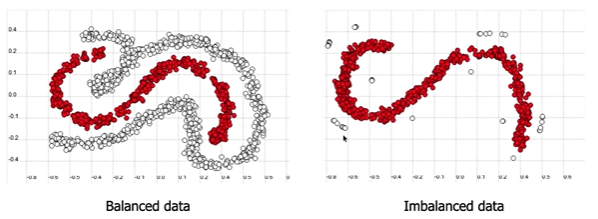
\includegraphics[width=0.7\textwidth]{images/imbalanced-balanced-data.png}
\end{center}

Two main approaches:
\begin{enumerate}
    \item Act on the data $\Rightarrow$ \textbf{Sampling methods}
    \item Act on the cost function $\Rightarrow$ \textbf{Cost-sensitive methods}
\end{enumerate}

\subsubsection{Sampling methods}

Compensate the lack of data by rebalancing the classes:

\begin{defnbox}[title=Oversampling — increase the minority class]
\textbf{What is it?} Generate new data inputs for the smallest class.

\textbf{Naive:} replicate data samples from the smallest class until balanced.

\textit{Drawback:} may lead to overfitting.

\medskip
\textbf{Smarter:} create new data samples based on neighboring existing ones (e.g.\ SMOTE).

\textit{Drawback:} may create noisy samples.

\begin{center}
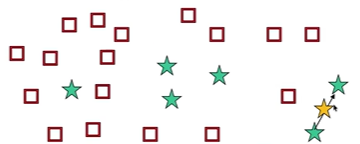
\includegraphics[width=0.48\textwidth]{images/oversampling.png}
\hfill
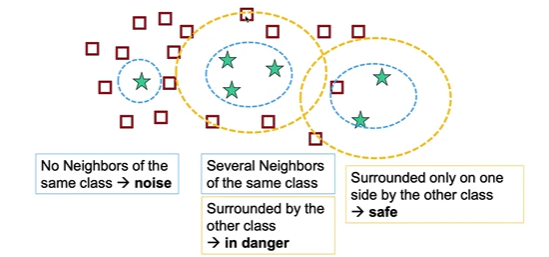
\includegraphics[width=0.48\textwidth]{images/oversampling2.png}
\end{center}
\end{defnbox}

\begin{defnbox}[title=Undersampling — reduce the majority class]
\textbf{What is it?} Remove redundant datapoints from the largest class.

\textbf{Naive:} randomly remove samples from the largest class until balanced.

\textit{Drawback:} may remove important samples.

\medskip
\textbf{Smarter:} remove only the redundant samples. Works well if the majority class is densely populated.

\begin{center}
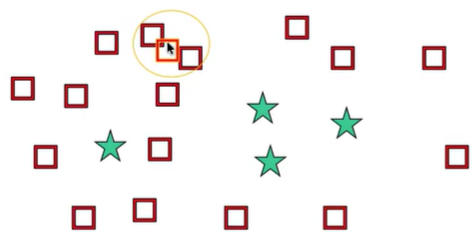
\includegraphics[width=0.6\textwidth]{images/undersampling.png}
\end{center}
\end{defnbox}

\subsubsection{Cost-sensitive methods}

Given $N$ training samples $\{(x_i, y_i)\}_{i=1}^N$, the standard empirical risk is:
\[
R({\mathbf{x}_i}, {y_i}, \mathbf{w}) = \frac{1}{N} \sum_{i=1}^{N} \ell(\hat{y}_i, y_i)
\]

A simple solution consists of \textbf{re-weighting} the samples to put more emphasis on the rare class:
\[
R({\mathbf{x}_i}, {y_i}, \mathbf{w}) = \frac{1}{N} \sum_{i=1}^{N} \beta_i \, \ell(\hat{y}_i, y_i)
\]

where $\beta_i$ is the weight of sample $i$, set \textbf{manually} (it cannot be optimized, as that would trivially give zero loss). It is chosen inversely proportional to the class frequency:
\[
\beta_i = 1 - \frac{N_k}{N}
\]
if sample $i$ belongs to class $k$, which contains $N_k$ samples (smaller class $\Rightarrow$ larger weight).

This re-weighting can be applied to any algorithm:

\begin{defnbox}[title=Weighted empirical risk — applications]
\textbf{Least-squares classification:}
\[
\min_{\mathbf{W}} \sum_{i=1}^{N} \beta_i \|\mathbf{W}^T \mathbf{x}_i - \mathbf{y}_i\|^2 + \lambda\|\mathbf{W}\|_F^2
\]

\textbf{Logistic regression:}
\[
\min_{\mathbf{w}} -\sum_{i=1}^{N} \beta_i \sum_{k=1}^{C} y_i^{(k)} \ln(\mathbf{w}^T \mathbf{x}_i)
\]

\textbf{SVM (soft-margin):}
\[
\min_{w^{(0)},\mathbf{\tilde{w}}} \;\tfrac{1}{2C}\|\mathbf{\tilde{w}}\|^2 + \sum_{i=1}^{N} \beta_i \max(0, 1 - y_i \cdot (w^{(0)} + \mathbf{\tilde{w}}^T \mathbf{x}_i))
\]
\end{defnbox}

\iffalse
% ------------------------------------------------------------
\newpage \section{Artificial neural networks (deep learning)}
% ------------------------------------------------------------

\begin{rembox}[title=Pourquoi et quand utiliser les réseaux de neurones ?]
\textbf{Pourquoi :} Les méthodes précédentes nécessitent de définir manuellement $\phi$ ou $k$. Les réseaux de neurones \textbf{apprennent automatiquement} une représentation des données adaptée au problème, couche par couche.

\vspace{0.3cm}

\textbf{Quand :} Grands datasets ; problèmes complexes avec des structures non-linéaires riches (images, texte, audio). En pratique, ils surpassent les méthodes précédentes dès que $N$ est suffisamment grand.

\vspace{0.3cm}

\textbf{Output :} Tout type de sortie selon la couche finale : $\hat{y} \in \mathbb{R}$ (régression), $\hat{y} \in (0,1)$ (classification binaire), distribution sur $C$ classes (classification multi-classe).
\end{rembox}

\vspace{0.6cm}

\subsection{Architecture}

Un réseau de neurones est composé de couches successives de transformations affines suivies de non-linéarités :

\[
h^{(0)} = x \quad \text{(input)}
\]
\[
h^{(l)} = \sigma\!\left(W^{(l)T} h^{(l-1)} + b^{(l)}\right) \quad l = 1, \dots, L
\]
\[
\hat{y} = h^{(L)} \quad \text{(output)}
\]

Avec :
\begin{itemize}
    \item $W^{(l)} \in \mathbb{R}^{d_{l-1} \times d_l}$ : poids de la couche $l$
    \item $b^{(l)} \in \mathbb{R}^{d_l}$ : biais de la couche $l$
    \item $\sigma$ : fonction d'activation non-linéaire
    \item $L$ : nombre de couches (profondeur du réseau)
\end{itemize}

\vspace{0.6cm}

\begin{defnbox}[title=Fonctions d'activation courantes]
\begin{itemize}
    \item \textbf{Sigmoid :} $\sigma(z) = \frac{1}{1+e^{-z}} \in (0,1)$ -- utilisée pour les sorties binaires.

    \item \textbf{ReLU :} $\sigma(z) = \max(0, z)$ -- la plus utilisée dans les couches cachées (évite le problème de vanishing gradient).

    \item \textbf{Softmax :} $\sigma(z)^{(k)} = \frac{e^{z^{(k)}}}{\sum_j e^{z^{(j)}}}$ -- utilisée en sortie pour la classification multi-classe.
\end{itemize}
\end{defnbox}

\vspace{0.6cm}

\subsection{Training -- Backpropagation}

La phase de training consiste à minimiser la loss function $R(W)$ par rapport à tous les paramètres $\{W^{(l)}, b^{(l)}\}$.

\vspace{0.4cm}

\begin{itemize}
    \item \textbf{Régression :} $R(W) = \frac{1}{N}\sum_i \|\hat{y}_i - y_i\|^2$

    \item \textbf{Classification :} $R(W) = -\frac{1}{N}\sum_i \sum_k y_i^{(k)} \ln \hat{y}_i^{(k)}$ (cross-entropy)
\end{itemize}

\vspace{0.5cm}

Le gradient $\nabla_{W^{(l)}} R$ est calculé par \textbf{backpropagation} : on propage l'erreur depuis la sortie vers l'entrée via la règle de la chaîne, couche par couche.

\vspace{0.4cm}

On utilise ensuite la descente de gradient (ou une variante comme \textbf{Adam}) :

\[
W^{(l)} \leftarrow W^{(l)} - \eta \, \nabla_{W^{(l)}} R
\]

\vspace{0.6cm}

\begin{rembox}[title=Stochastic Gradient Descent (SGD)]
Plutôt que de calculer le gradient sur tout le dataset (coûteux), on estime le gradient sur un \textbf{mini-batch} de $B$ samples à chaque itération. Cela accélère l'entraînement et permet de traiter de grands datasets.
\end{rembox}
\fi
% ============================================================
\chapter{Unsupervised ML}
% ============================================================

\section{Dimensionality reduction}

\newpage \section{k-Means Clustering}

















\vspace{8cm}


























% ------------------------------------------------------------
\newpage \section{Introduction to multilayer perceptron model (MLP)}
% ------------------------------------------------------------

\subsection{Parametric feature expansion}
Maintenant que on a vu que on peut faire des algorithms, des trainings plus compliqués mais aussi plus précis en ajoutant des bias, puis on a régularisé, puis on a mis des sécurité pour éviter l'underflow ou encore on a fait du polynomial feature expansion qui nous permettait de tester différentes manières de prendre un sample et de travailler avec des combinaisons, des puissances des éléments du vecteur d'un même input et de le pousser plus loin et plus facilement avec les kernel methods.

\medskip

Maintenant tout ça c'est bien sympa mais on veut aller encore plus loin et faire un peu mieux quand même, ajouter encore de la précision, là où le polynomial feature expansion nous permettait de suivre, d'approximer une courbe, là on va vouloir approximer plus, grand, plus complexe (l'exemple de la heatmap).

\medskip

Concrement, on veut faire du linéaire du non-linéaire, mais on ne veut pas faire du polynomial feature expansion manuellement. De manière plus intelligente, on va faire apprendre à notre modèle le meilleur feature expansion possible aussi.

\bigskip

En fait on va appliquer un modèle linéaire, puis ajouter de la non-linearity avec la fonction et ensuite on va résoudre comme linéairement.

\medskip

D'abord on définit pour nous aider à simplifier plus tard :

\[
a_{(1)}
= W_{(1)}^T
\begin{pmatrix} 1 \\ x \end{pmatrix}
= \begin{pmatrix}
W_{(1)}^{(1,0)} + W_{(1)}^{(1,1)} x \\
\vdots \\
W_{(1)}^{(M,0)} + W_{(1)}^{(M,1)} x
\end{pmatrix}
= \begin{pmatrix}
a_{(1)}^{(1)} \\
\vdots \\
a_{(1)}^{(M)}
\end{pmatrix}
\in \mathbb{R}^{M \times 1}
\]

Alors on va définir notre parametric feature expansion qui va revenir à appliquer une fonction sur les résultats du produit $W$ et $x$ soit :

\[
x
\rightarrow
z_{(1)} =
\begin{bmatrix}
f\!\left(a_{(1)}^{(1)}\right) \\
\vdots \\
f\!\left(a_{(1)}^{(M)}\right)
\end{bmatrix}
=
f\!\left(
W_{(1)}^T
\begin{pmatrix}
1 \\
x
\end{pmatrix}
\right)
\in \mathbb{R}^{M \times 1}
\]

Avec :
\begin{itemize}
    \item $f$ the activation function (ex: sigmoid, hyperbolic tangent...)
    \item $M$ the number of hidden units (the dimension of the hidden representation)
    \item $W_{(1)}$ the weights of the first layer (the parameters of the feature expansion)
    \item $z$ the hidden representation (the output of the feature expansion)
\end{itemize}

\medskip

Par conséquent, avec ces changements on a :

\begin{align*}
\hat{y}
&=
w_{(2)}^{T} z_{(1)}
=
\sum_{i=1}^{M}
w^{(i)}_{(2)}
f\left(
W^{(i,0)}_{(1)}
+
W^{(i,1)}_{(1)}x
\right)
\end{align*}

\begin{defnbox}[title=Universal approximation]
We can approximate any continuous function with a linear combination of translated/scaled ReLU functions $f(\cdot)$
\end{defnbox}
Maintenant, on peut étendre la formule pour montrer un peu à quoi ça ressemble un peu comme Taylor ou Fourier...

\begin{minipage}{0.58\textwidth}
\begin{align*}
\hat{y}
&=
w_{(2)}^{T} z_{(1)}
=
\sum_{i=1}^{M}
w^{(i)}_{(2)}
f\left(
W^{(i,0)}_{(1)}
+
W^{(i,1)}_{(1)}x
\right)
\\[6pt]
&=
w^{(1)}_{(2)}
f\left(
W^{(1,0)}_{(1)}
+
W^{(1,1)}_{(1)}x
\right)
\\[6pt]
&\quad+
w^{(2)}_{(2)}
f\left(
W^{(2,0)}_{(1)}
+
W^{(2,1)}_{(1)}x
\right)
\\[6pt]
&\quad+
w^{(3)}_{(2)}
f\left(
W^{(3,0)}_{(1)}
+
W^{(3,1)}_{(1)}x
\right)
+
\cdots
\end{align*}
\end{minipage}
\hfill
\begin{minipage}{0.3\textwidth}
\centering
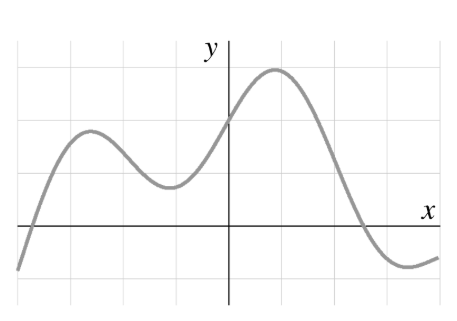
\includegraphics[width=\textwidth]{images/universal-appro-before.png}

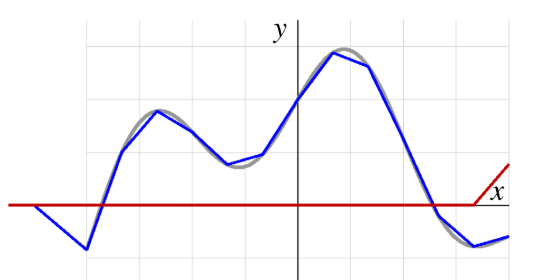
\includegraphics[width=\textwidth]{images/universal-appro-after.png}
\end{minipage}

\subsection{Dealing with D > 1}
Dans la majorité des cas il y a plusieurs features, comment faire ?
\[
a_{(1)} = W_{(1)}^T
\begin{pmatrix}1 \\ x_1 \\ \vdots \\ x_D\end{pmatrix}
\in \mathbb{R}^{M \times 1} \quad\text{and}\quad
z_{(1)} = f\!\left(a_{(1)}\right) \in \mathbb{R}^{M \times 1}
\] 

\subsection{Dealing with C > 1}
De même, généralement, plusieurs output sont calculées, comment faire ? On va remplacer $w_{(2)}$ par une matrice $W_{(2)} \in \mathbb{R}^{M \times C}$.
\[\hat{y} = W_{(2)}^T z_{(1)} \in \mathbb{R}^{C \times 1}\]

The resulting simple artifical neural network with one hidden layer can be depicted as shown below:
\begin{center}
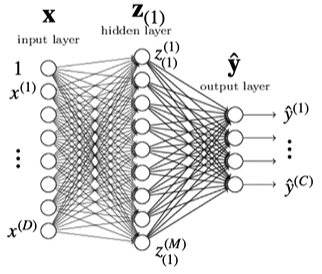
\includegraphics[width=0.4\textwidth]{images/simple-artifical-nn.png}
\end{center}

\subsection{Multilayer perceptron (MLP)}
Maintenant, si on veut ajouter encore certaines fonctions, certaines non-linearity, certaines précision, on peu cumuler les couches, les étapes intermédiaires de notre neural network, pour ça, c'est très simple, il suffit de répéter l'opération simplement :

\[
z_{(1)}
=
f
\left(
W^{(1)T} x
\right)
\]

\[
z_{(l)}
=
f
\left(
W_{(l)}^{T} z_{(l-1)}
\right)
\]

We call going from $x$ to $y$ the \textbf{forward pass} of the network.

\subsection{Training}

For the regression la loss function will be:

\[
R(W)
=
\frac{1}{N}
\sum_{i=1}^{N}
\|
\hat{y}_i(W) - y_i
\|^2
\]

In that case to solve it we will be using graident descent and the gradient will be an average of gradients as the empirical risk is an average over the training.

\[
R(\{W^{(1)}\})
=
\frac{1}{N}
\sum_{i=1}^{N}
\ell(\hat{y}_i, y_i)
=
\frac{1}{N}
\sum_{i=1}^{N}
\ell_i
\]

\medskip

For the $k$th dimension of the output layer $l$ we will have :

\[
a_{(k)}^{(l)}
=
\sum_{j}
W_{(k,j)}^{(l)}
z_{(j)}^{(l-1)}
\]

The form for the partial derivative of $a$ is:

\[
\frac{
\partial a^{(k)}_{(l)}
}{
\partial W^{(k,j)}_{(l)}
}
=
z^{(j)}_{(l-1)}
\]

Moreover we define to simplify :

\[
\delta^{(k)}_{(l)}
=
\frac{
\partial \ell_i
}{
\partial a^{(k)}_{(l)}
}
\]

Consequently:, using chain rule:

\[
\frac{
\partial \ell_i
}{
\partial W_{(k,j)}^{(l)}
}
=
\delta_{(k)}^{(l)}
z_{(j)}^{(l-1)}
\]

And for the last layer we will have

\[
a_{(k)}^{(L)}
=
\hat{y}^{(k)}
\]

Meaning that we can also go back from last $\delta^{(L)}$ to the previous ones (because we didn't exactly know all the values, and weights and factors)

\[
\frac{
\partial \ell_i
}{
\partial W_{(l)}^{(k,j)}
}
=
\delta_{(l)}^{(k)}
z_{(l-1)}^{(j)}
\]

Tzzo go back we will use a special algorithm \textbf{BACK PROPAGATION!!!!}

\bigskip

\begin{algbox}[title=Back propagation]
\begin{enumerate}
    \item Propagate $x_i$ forward through the network (using gradient descent)

    \item Compute $\delta^{(L)}$ depending on the loss

    \item Propagate that delta backward to obtain each $\delta^{(l)}$

    \item At each layer, compute the partial derivatives:

    \[
    \frac{
    \partial \ell_i
    }{
    \partial W_{(l)}^{(k,j)}
    }
    =
    \delta_{(l)}^{(k)}
    z_{(l-1)}^{(j)}
    \]
\end{enumerate}
\end{algbox}





\subsection{Stochastic gradient descent}

On va avoir des adaptations du gradient descent pour pouvoir le  corroborrer à notre problème.

\[
\text{inspired by the gradient descent -- the gradient is sample in each iteration.}
\]

\[
W_k \leftarrow W_{k-1} - \eta \nabla \ell_{i(k)}(W_{k-1})
\]

\[
\Rightarrow \text{but has problems with jumps as } i \text{ obtain a more reliable}
\]
\[
\text{gradient estimate, SGD with mini-batches of } B \text{ examples}
\]

\[
W_k \leftarrow W_{k-1} - \eta \sum_{b=1}^{B} \nabla \ell_{(b,k)}(W_{k-1})
\]

\bigskip

\textbf{SGD extensions}

\[
\text{momentum } \Rightarrow \text{ add inertia the parameter updates}
\]

\[
\nu \leftarrow \gamma \nu + \eta\nabla R(W)
\]

\[
W \leftarrow W - \nu
\]

\[
\text{with } \gamma>0 \Rightarrow \text{ accelerates if the gradient does not change too much}
\]

\textbf{For classification}

We can use the softmax.

\[
\hat{y}^{(k)} =
\frac{
\exp\left(w_{(L)}^T(k)\, z_{(L-1)}\right)
}{
\sum_{j=1}^{C}
\exp\left(w_{(L)(j)}^T\, z_{(L-1)}\right)
}
\]

\[
w_{(L)j} \text{ : column of } W_{(L)}
\]

In this case:

\[
R(W) := - \frac{1}{N}
\sum_{i=1}^{N} \sum_{j=1}^{C}
y_{i}^(k) \log \hat{y}^{(k)}_j
\]


































\end{document}
